\documentclass[a4paper, twoside]{article}

%\usepackage{fixltx2e}
\usepackage{graphicx}
\usepackage{listings}
\lstset{tabsize=2, breaklines=true, breakatwhitespace=true, basicstyle=\ttfamily}

\setlength{\oddsidemargin}{0in} \setlength{\evensidemargin}{0in}
\setlength{\textwidth}{6.2in}
\setlength{\topmargin}{-0.3in} \setlength{\textheight}{9.8in}

\title{CS22510 Assignment - Runners and Riders}
\author{Tom Leaman (thl5)}

\begin{document}
\maketitle
\newpage
\tableofcontents
\newpage

\section{Event Creator}
\subsection{Source code}
\subsubsection{main.cpp}
\lstinputlisting{../event_creator/main.cpp}
\subsubsection{Makefile}
\lstinputlisting{../event_creator/Makefile}
\subsection{Compiler output}
%TODO
\subsection{Example usage}
%TODO
\subsection{Generated files}
%TODO

\section{Checkpoint Manager}
\subsection{Source code}
\subsubsection{event/Course.java}
\lstinputlisting{../checkpoint_manager/src/event/Course.java}
\subsubsection{event/Entrant.java}
\lstinputlisting{../checkpoint_manager/src/event/Entrant.java}
\subsubsection{event/Event.java}
\lstinputlisting{../checkpoint_manager/src/event/Event.java}
\subsubsection{event/node/Node.java}
\lstinputlisting{../checkpoint_manager/src/event/node/Node.java}
\subsubsection{event/node/CheckpointNode.java}
\lstinputlisting{../checkpoint_manager/src/event/node/CheckpointNode.java}
\subsubsection{event/node/JunctionNode.java}
\lstinputlisting{../checkpoint_manager/src/event/node/JunctionNode.java}
\subsubsection{event/node/MedicalcheckpointNode.java}
\lstinputlisting{../checkpoint_manager/src/event/node/MedicalCheckpointNode.java}
\subsubsection{event/update/ArrivalUpdate.java}
\lstinputlisting{../checkpoint_manager/src/event/update/ArrivalUpdate.java}
\subsubsection{event/update/DepartureUpdate.java}
\lstinputlisting{../checkpoint_manager/src/event/update/DepartureUpdate.java}
\subsubsection{event/update/ExcludedUpdate.java}
\lstinputlisting{../checkpoint_manager/src/event/update/ExcludedUpdate.java}
\subsubsection{event/update/InvalidUpdate.java}
\lstinputlisting{../checkpoint_manager/src/event/update/InvalidUpdate.java}
\subsubsection{event/update/TimeUpdate.java}
\lstinputlisting{../checkpoint_manager/src/event/update/TimeUpdate.java}
\subsubsection{event/update/Update.java}
\lstinputlisting{../checkpoint_manager/src/event/update/Update.java}
\subsubsection{event/gui/CheckpointPanel.java}
\lstinputlisting{../checkpoint_manager/src/gui/CheckpointPanel.java}
\subsubsection{event/gui/Driver.java}
\lstinputlisting{../checkpoint_manager/src/gui/Driver.java}
\subsubsection{event/util/FileIO.java}
\lstinputlisting{../checkpoint_manager/src/util/FileIO.java}
\subsubsection{event/util/Parser.java}
\lstinputlisting{../checkpoint_manager/src/util/Parser.java}
\subsubsection{event/util/Time.java}
\lstinputlisting{../checkpoint_manager/src/util/Time.java}
\subsection{Compiler output}
\lstset{tabsize=2, breaklines=true, breakatwhitespace=false, basicstyle=\ttfamily}
\lstinputlisting{checkpoint_manager_compilation.txt}
\lstset{tabsize=2, breaklines=true, breakatwhitespace=true, basicstyle=\ttfamily}
\subsection{Example usage}
\subsubsection{Checkpoint logging}
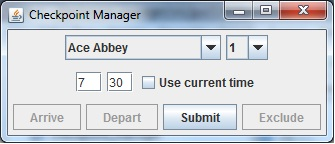
\includegraphics{screenshot1.jpg}
\subsubsection{Arriving at a medical checkpoint}
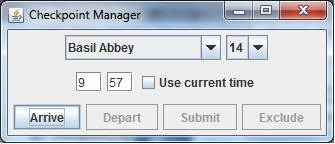
\includegraphics{screenshot2.jpg}
\subsubsection{Departing a medical checkpoint}
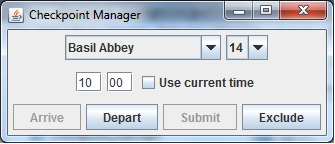
\includegraphics{screenshot3.jpg}
\subsubsection{File locking}
%TODO

\section{Event Manager}
\subsection{Compiler output}
\lstinputlisting{event_manager_compilation.txt}
\subsection{Example usage \& results listing}
\lstinputlisting{event_manager_output.txt}
\subsection{Generated log file}
\lstinputlisting{example_log.txt}

\section{Program descriptions}
\subsection{Event Creator}
The Event Creator program has been implemented in C++. It allows the user to
create a new event, add competitors to an event and create courses for an event.
It does virtually no error checking (it will crash if it is given the wrong
format for data e.g. a string instead of an int). I feel this is its greatest
short-coming.
\subsection{Checkpoint Manager}
The Checkpoint Manager has been implemented in Java and makes use of the Swing
framework. It allows the user to update the location of an entrant and performs
very simple error checking to ensure that an entrant cannot be logged as
arriving at a medical checkpoint twice, for example. It includes an option to
use the current time for each update. It locks both the times file and log file
when writing.
\subsection{Event Manager}
The Event Manager has been implemented in C (based on the previous CS237
assignment). It allows the user to query the status of an individual entrant,
list entrants in various states of competition and list the results (in sorted
format). It also locks the log file when writing.

\end{document}
